%%%%%%%%%%%%%%%%%%%%%%%%%%%%%%%%%%%%%%%%%%%%%%%%%%%%%%%%%%%
% --------------------------------------------------------
% Tau
% LaTeX Template
% Version 2.4.1 (22/05/2024)
%
% Author: 
% Guillermo Jimenez (memo.notess1@gmail.com)
% 
% License:
% Creative Commons CC BY 4.0
% --------------------------------------------------------
%%%%%%%%%%%%%%%%%%%%%%%%%%%%%%%%%%%%%%%%%%%%%%%%%%%%%%%%%%%
\documentclass[9pt,a4paper,twoside]{tau-class/tau}

%----------------------------------------------------------
% TITLE
%----------------------------------------------------------

\journalname{ESCOM}
\title{Cellular Automata}

%----------------------------------------------------------
% AUTHORS, AFFILIATIONS AND PROFESSOR
%----------------------------------------------------------

\author[a]{Diego Castillo Reyes}
\author[a]{Marthon Leobardo Yañez Martinez}
\author[a]{Aldo Escamilla Resendiz}
\author[a]{Muñoz González Eduardo}

%----------------------------------------------------------

\affil[a]{Researcher}


\professor{Dra. Miriam Pescador Rojas}

%----------------------------------------------------------
% FOOTER INFORMATION
%----------------------------------------------------------

\institution{Escuela Superior de Cómputo, IPN}
\footinfo{Cellular Automata}
\theday{June 21, 2024}
\course{Genetic Algorithms}

%----------------------------------------------------------
% ABSTRACT AND KEYWORDS
%----------------------------------------------------------

\begin{abstract}    
    Cellular automata are a mathematical and computational model used to simulate dynamic systems. 
        This work presents a review of cellular automata, their history, classification, and applications. 
        Additionally, an example of one-dimensional and two-dimensional cellular automata is shown.
\end{abstract}

%----------------------------------------------------------

\keywords{Automata, Cellular, Genetic, Algorithms, Simulation}

%----------------------------------------------------------

\begin{document}
		
    \maketitle 
    \thispagestyle{firststyle} \tauabstract
    \tableofcontents
%----------------------------------------------------------

\section{Introduction}

    \section{Cellular Automata}

    Cellular automata (CA) are \textit{discrete, abstract computational systems} that have proved useful both as general models of complexity and as more specific representations of non-linear dynamics in a variety of scientific fields. 

    Firstly, CA are typically spatially and temporally discrete. They are composed of a finite or denumerable set of homogeneous, simple units called cells. At each time unit, the cells instantiate one of a finite set of states. 
    They evolve in parallel at discrete time steps, following state update functions or dynamical transition rules. 
    The update of a cell's state is obtained by taking into account the states of cells in its local neighborhood, meaning there are no actions at a distance.

    Secondly, CA are abstract. They can be specified in purely mathematical terms, and physical structures can implement them.

    Thirdly, CA are computational systems. They can compute functions and solve algorithmic problems. Despite functioning differently from traditional 
    Turing machine-like devices, CA with suitable rules can emulate a universal Turing machine\footnote{\cite[Read more at:  "Turing Machines", The Stanford Encyclopedia of Philosophy (Winter 2021 Edition), Edward N. Zalta (ed.), URL = <https://plato.stanford.edu/archives/win2021/entries/turing-machine/>.]{sep-touring-machine}}, 
    and therefore compute anything that is computable according to Turing's thesis.\cite{sep-cellular-automata}


\section{Background}


    The concept of cellular automata was invented by Stansilaw Ulam and John Von Neumann in
    the 1940s while they were working at the Los Alamos National Laboratory.
    The work on cellular automata began in the 1940s, with significant developments occuring throughout
    that decade. Von Neumann’s comprehensive work on self-replicating automata was published 
    posthumously in 1966 in the book "Theory of Self-Reproducing Automata," edited by 
    Arthur W. Burks.

    A cellular automaton (CA) is a one-dimensional array (which can be infinitely long in both directions) of cells. 
    Time progresses in discrete steps, and at each step, every cell is in one of a finite number of possible states. The state of each cell changes at each tick of the clock, and this new state is determined entirely by the current state of the cell and its immediate left and right neighbors. 
    This state change is governed by a function called the local rule, which is identical for all cells. 
    The CA operates autonomously without any external input. 
    The collection of all cell states at any given time is referred to as the configuration or global state of the CA, 
    representing its stage of evolution. Starting from an initial configuration at time t = 0, the CA evolves deterministically according to the local rule applied to each cell at each clock tick. (see Fig. \ref{fig:timeStep})

    When the local rule is applied to each cell, it transforms the entire set of configurations into itself. 
    This transformation is known as the global map or global rule of the CA. This description captures the essence of a CA, which is a widely studied structure.
    \begin{figure}[H]
        \centering
        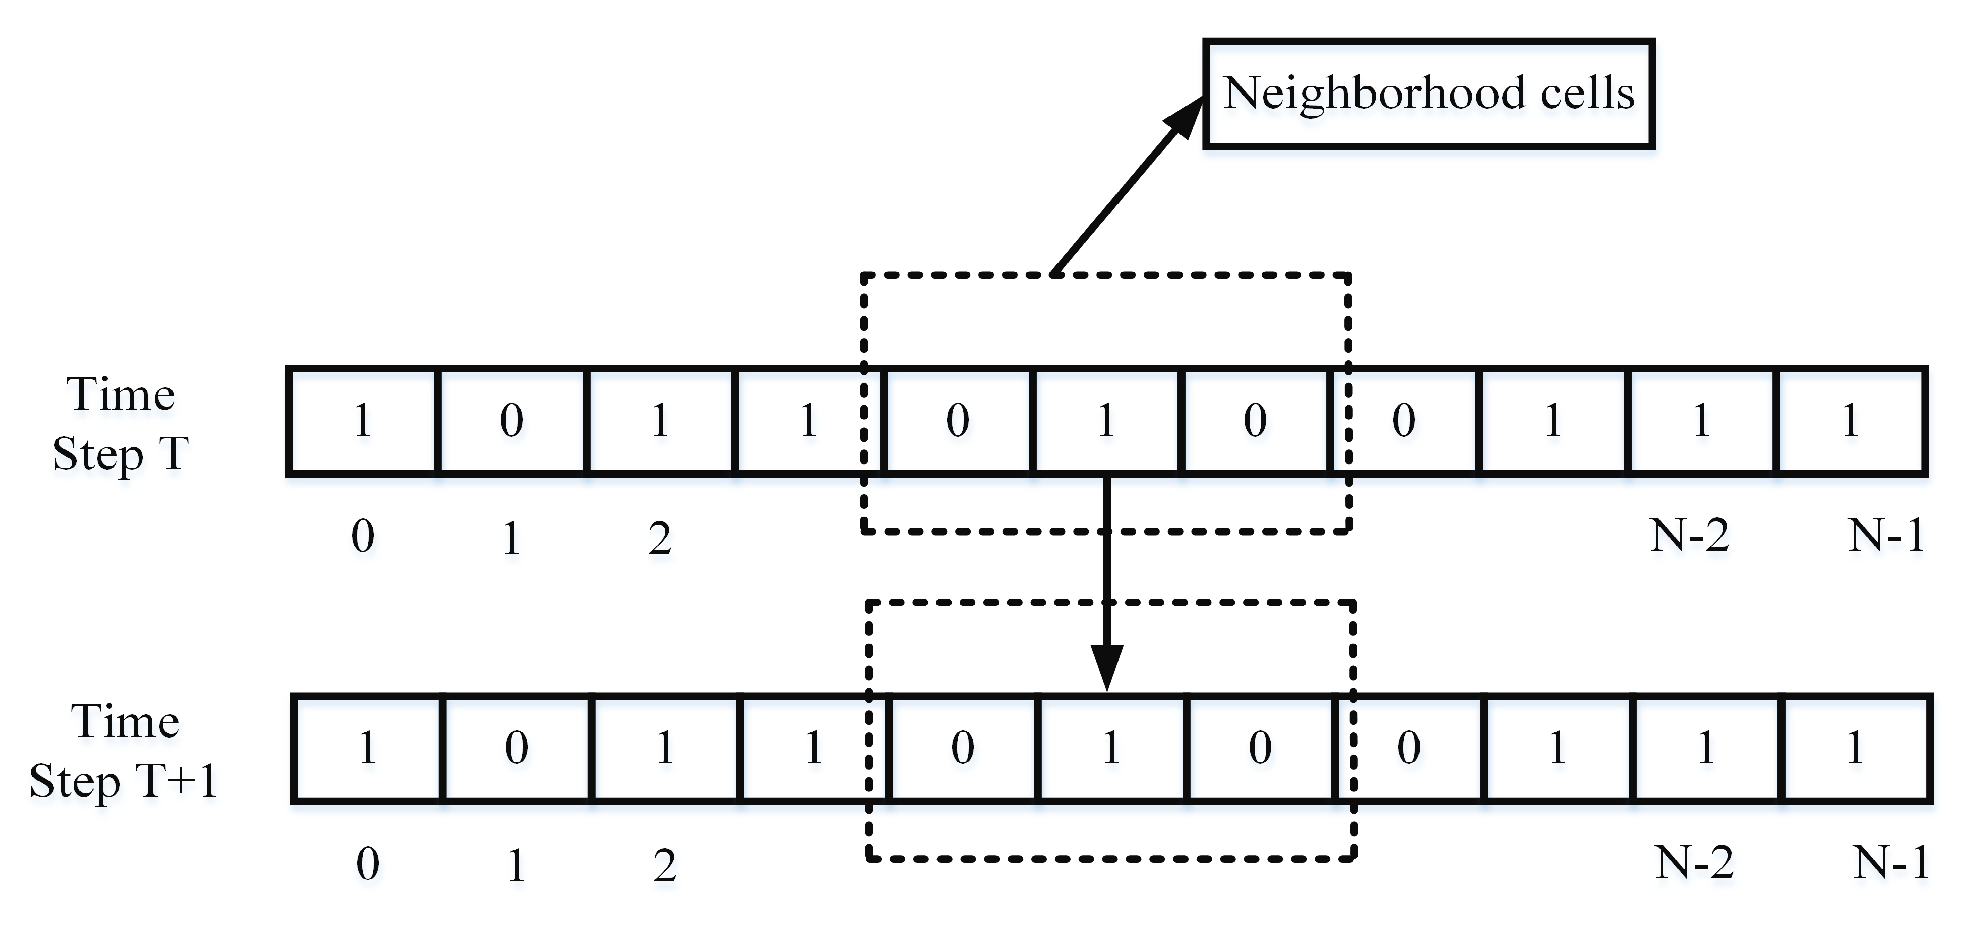
\includegraphics[width=0.75\columnwidth]{figures/timestep.png}
        \caption{Evolution of a CA at each time step. \cite{math11102322} }
        \label{fig:timeStep}
    \end{figure}

    The automaton initially described by von Neumann\cite{von-neumann-automata} consists of a two-dimensional infinite array of uniform cells, with each cell connected to its four orthogonal neighbors. 
    This structure was originally termed a cellular space, though the term CA is now more commonly used. Von Neumann introduced this concept as a formal model for self-reproducing biological systems. His key ideas can be traced back to his earlier work on modeling biological systems. 
    Von Neumann aimed to apply the rigor of axiomatic and deductive methods to the study of complex natural systems. His concept of a self-reproducing automaton is a remarkable adaptation of the idea behind constructing a universal Turing Machine (TM).

    \begin{figure}[H]
        \centering
        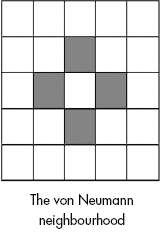
\includegraphics[width=0.75\columnwidth]{figures/vonNeumann.png}
        \caption{Von Neumann's cellular automaton.}
        \label{fig:vonNeumann}
    \end{figure}



    \subsection{Motivation}
    
    
    Cellular automata, a concept derived from computer science, are increasingly employed as models in ecological research. This concept spans a variety of topics, including automata theory and artificial intelligence. 
    Cellular automata, as representations of this concept, create miniature worlds where each cell houses an automaton. The behavior of a cellular automaton can be remarkably complex, often resembling lifelike processes. 
    This complexity has inspired a new field of study known as artificial life or, more cautiously, complex systems. Conferences in this field attract computer and mathematical scientists, as well as a growing number of participants from geography, ecology, geology, and other disciplines, along with a popular audience. 
    Currently, the field of ecology has accumulated sufficient experience with cellular automaton models to move beyond initial simple models and harness the full potential of this tool for comprehensive simulation. 
    However, validation and interpretation continue to be significant challenges in utilizing these models effectively.\cite{DEWDNEY2008541}

    The primary motivation behind cellular automata was to understand and model complex
    systems using simple, local rules. This idea was rooted in the study of biological 
    processes and the desire to create self-replicating machines.

    \subsection{Developments}
    \begin{itemize}
        \item Conway's Game of Life (1970): British mathematician John Conway popularized cellular
        automata with his "Game of Life", a bidimensional binary cellular automaton. 
        This game demonstrated how simple rules could lead to complex emergent behavior, 
        sparking widespread interest and research in cellular automata.

        \item Stephen Wolfram's work (1980s): Wolfram conducted extensive research on cellular
        automata, classifying them into four types based on their behavior and demonstrating 
        their potential as models of natural processes and as computational systems.
    \end{itemize}

    Fig. \ref{fig:figure} An example of Conway's Game of Life.
	\begin{figure}[H]
		\centering
		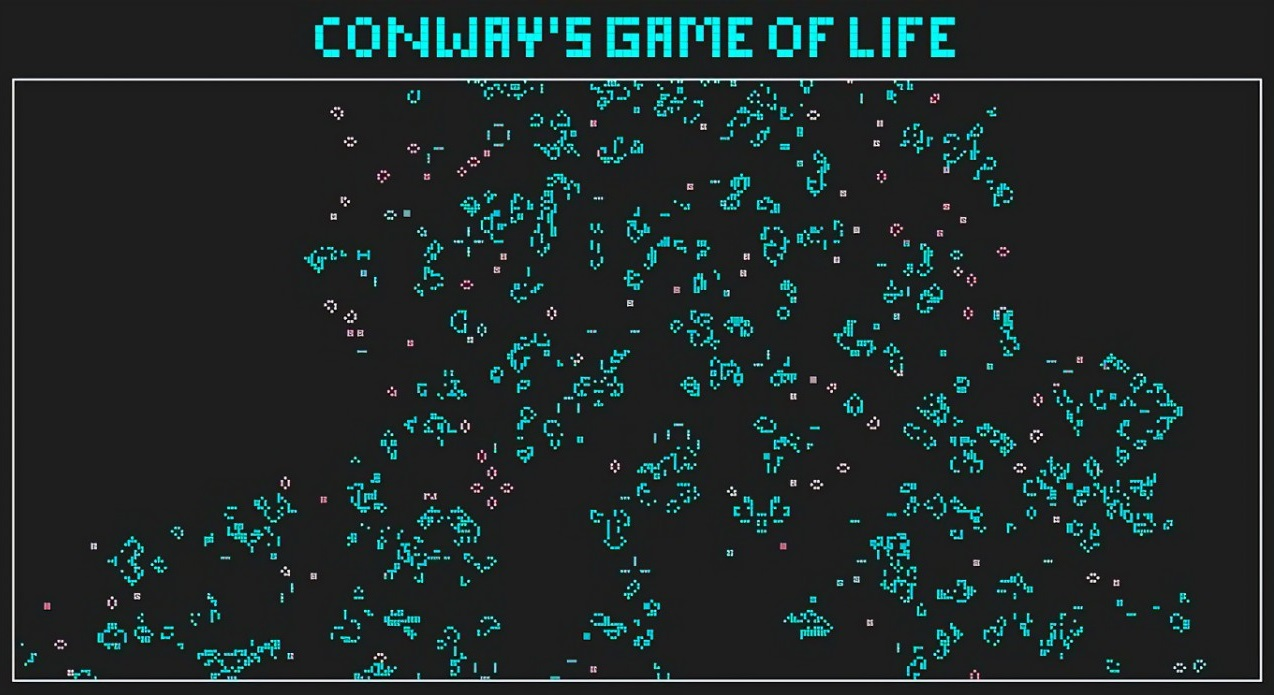
\includegraphics[width=0.75\columnwidth]{figures/gameOfLife.jpg}
		\caption{Conway's Game of Life.}
		\label{fig:figure}
	\end{figure}

    \subsection{Applications}
	
        Cellular automata have been used in various fields, including:
        
        \begin{itemize}
            \item Computer Science: Parallel computation, cryptography, and image processing.
            \item Physics: Modeling physical systems, such as fluid dynamics and crystal growth.
            \item Biology: Simulating biological processes, such as population dynamics and pattern formation.
        \end{itemize}
		
        Fig. \ref{fig:ExampleAutonoma} Application of cellular automata on Computer Science.
	\begin{figure}[H]
		\centering
		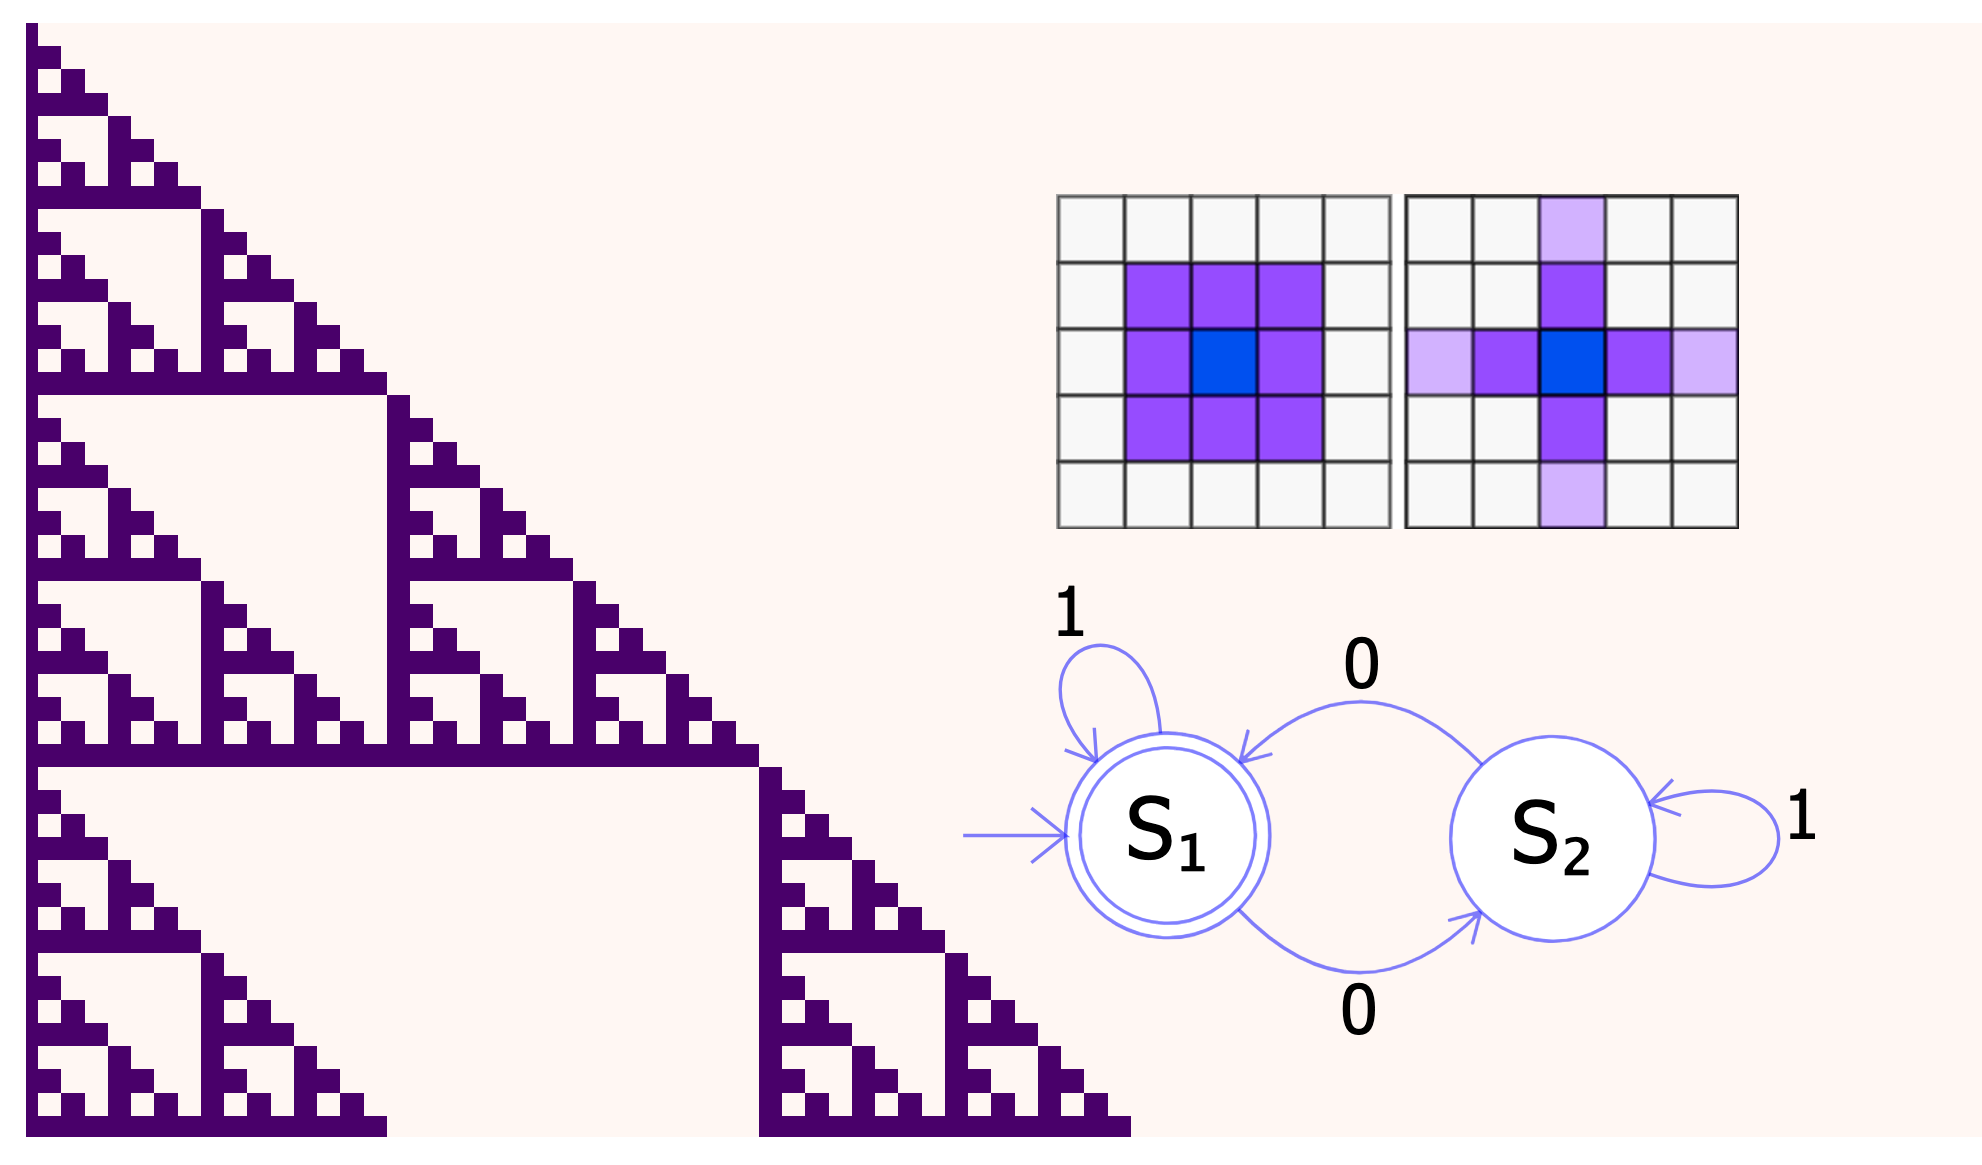
\includegraphics[width=0.75\columnwidth]{figures/theoryOfComputation.png}
		\caption{Example of cellular automata.}
		\label{fig:ExampleAutonoma}
	\end{figure}

\section{Cellular Automata Algorithm}
    \begin{algorithm}
        \caption{Basic Cellular Automaton}
        \KwIn{\texttt{gridWidth}: Width of the grid, \texttt{gridHeight}: Height of the grid, \texttt{states}: Set of possibles states for the cells, \texttt{neighborhood}: Set of relative positions defining the neighborhood of each cell, \texttt{rules}: Set of state transition rules, \texttt{maxTimeSteps}: Maximum number of time steps}
        \KwOut{The final state of the grid}
        
        Initialize \texttt{gridHeight} $\times$ \texttt{gridWidth}, set the initial states on the grid and create \texttt{newGrid} as a copy of the grid.\;
        
        \While{$i$ < \texttt{maxTimeSteps}}{
            \For{$x$ in \texttt{gridWidth}}{
                \For{$y$ in \texttt{gridHeight}}{
                    \texttt{neighbors} = getNeighbors(\texttt{grid}, \texttt{neighborhood}, $x$, $y$)\;
                    \texttt{newGrid}[$x$][$y$] = applyRules(\texttt{grid}[$x$][$y$], \texttt{neighbors}, \texttt{rules})\;
                }
            }
            Display the state of \texttt{newGrid}
            \texttt{grid} = \texttt{newGrid}\;
            $i$++\;
        }
        \end{algorithm}

\section{Parameters Required on a Cellular Automata}

\section{Versions of Cellular Automata}

\section{Analogy with the Nature}
    
\section{Implementation Repositories}

\section{Usage Examples}


\addcontentsline{toc}{section}{References}
\printbibliography

\end{document}